%************************************************
\myChapter{Metoda}\label{ch:method}
%************************************************

W tym rozdziale przedstawię metodę wykorzystaną do określania pozycji obiektów znajdujących się w ramce.\\

Ramka składa się z dwudziestu modułów, każdy z nich zawiera jedną diodę LED oraz 8 fotodiod.

Podczas działania urządzenia zapalane są kolejno moduły ponumerowane od 0 do 19, układ jest zaprojektowany w taki sposób, aby w dowolnej chwili świecił się najwyżej jeden moduł. W czasie świecenia wybierane są moduły leżące po przeciwnej stronie i odczytywany jest ich stan, który następnie trafi do komputera. Host decyduje o tym które moduły należy zapalić, odpytać oraz w jakiej kolejności to zrobić. Mikrokontroler jest jednostką wykonawczą tych poleceń i dostarcza z powrotem dane w postaci wygodnej do analizy.

Na potrzeby pracy przyjmijmy, że światło z nadajnika rozchodzi się w postaci dyskretnych promieni \pauza wiązek światła łączących go z odbiornikami. Pozwala to na uproszczenie opisu metody działania bez poświęcania dokładności \pauza światło, które nie trafia w aktywną w danej chwili fotodiodę nie jest brane pod uwagę.

Przerwanie któregokolwiek z takich promieni poprzez zasłonięcie odbiornika powoduje zmianę stanu na jego wyjściu. Fotodiody oświetlone dają na wyjściu stan niski, zaś nieoświetlone \ppauza wysoki.

Rysunek~\ref{fig:scene_rays_sample} prezentuje schemat ramki z włączonym jednym modułem.

\begin{figure}
 %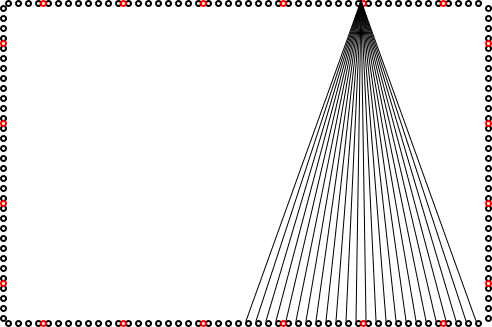
\includegraphics[width=\textwidth]{gfx/scene_rays_sample.svg}
 \input{gfx/scene_rays_sample.pdf_tex}
 \caption{Wizualizacja ramki. Czarne okręgi \ppauza fotodiody; czerwone \ppauza diody LED; czarne odcinki \ppauza odbierane promienie.}
 \label{fig:scene_rays_sample}
\end{figure}